\chapter{Relação entre Classes $B_1$-EPG, EPT e VPT}

\begin{flushright}
\begin{minipage}[t][0cm][b]{0.47\textwidth}
\emph{
A Matemática não mente. Mente quem faz mau uso dela.}
\end{minipage}

\rule[0cm]{7cm}{0.03cm}%{largura}{espessura}

Albert Einstein
\end{flushright}


\section{Introduction}

Models based on paths intersection  may consider  intersections by vertices or   intersections by edges.  Cases where the paths are hosted on a tree  appear first in the literature, see for instance \cite{gavril1978recognition, golumbic1985edge, golumbic1985}.  Representations using paths on a grid were considered later, see  \cite{golumbic2009,golumbic2013, golumbic2013intersection}. %More details on each intersection model will be given in the following text.

 Let $P$ be a family of paths on a host tree $T$ . Two types of intersection graphs from the pair $<P,T>$ are defined, namely VPT and EPT graphs.
The \textit{edge intersection graph} of $P$, EPT(P), has vertices which correspond to the members of $P$, and two vertices are adjacent in EPT(P) if and only if the corresponding paths in $P$ share at least one edge in T. Similarly, the \textit{vertex intersection graph} of $P$, VPT(P), has vertices which correspond to the members of $P$, and two vertices are adjacent in VPT(P) if and only if the corresponding paths in $P$ share at least one vertex in $T$.
%
VPT and EPT graphs are incomparable families of graphs. However, when the maximum degree of the host tree is restricted to three the family of
VPT graphs coincides with the family of EPT graphs \cite{golumbic1985edge% \cite{alcon2010necessary
}. Also it is known that any Chordal EPT graph is VPT (see~\cite{syslo1985triangulated}). Recall that it was shown that Chordal graphs are the vertex intersection graphs of subtrees of a tree \cite{gavril1974intersection}.


Edge intersection graphs of paths on a grid are called \textit{EPG graphs}. 

In \cite{golumbic2009}, the authors proved that every graph is EPG, and started the study of the subclasses
defined by bounding the number of times any path used in the representation can bend.  Graphs admitting a representation
where  paths  have at most $k$ changes of direction  (bends) were called $B_k$-EPG. 
 In particular, when the paths have at most one bend we have the \textit{ $B_1$-EPG graphs} or a \textit{single bend EPG graphs}.

 A pertinent question in the context of path intersection graphs is as follows: given two classes of path intersection graphs,
 the first whose host is a tree and the second whose host is a grid,  is there an intersection or containment relationship among these classes? What do we know about it?

In the present paper we will explore $B_1$-EPG graphs, in particular diamond-free graphs and Chordal graphs. We will work on the question about the containment
relation between  VPT, EPT and $B_1$-EPG graph classes.


 A collection  of sets satisfies the \textit{Helly property} when every pair-wise intersecting sub-collection  has at least one common element. When this property
 is satisfied by the set of vertices (edges) of the paths used in a representation, we get a Helly representation.  Helly $B_1$-EPG graphs were studied
 in \cite{bornstein2019complexity}.                                     
It is known that not every $B_1$-EPG graph admits a Helly $B_1$-EPG representation. We are interested in determining the subgraphs that make
$B_1$-EPG graphs do not admit a Helly representation. In the present work, we describe some structures that will be present in any such subgraph,
and, in addition, we present new  Helly $B_1$-EPG  subclasses.
Moreover,  we  describe new  Helly $B_1$-EPG  subclasses % that have Helly property 
and we give some sets of subgraphs that delimit Helly subfamilies.   
\section{Definitions and Technical Results}

The \textit{vertex set} and the \textit{edge set} of a graph $G$ are denoted by $V(G)$ and $E(G)$, respectively.  Given a vertex $v\in V(G)$,  $N(v)$ and $N[v]$ represent the open and the close
 \textit{neighborhood} of $v$ in $G$, respectively. 
For a subset $S \subseteq V(G)$,  $G[S]$ is the subgraph of $G$ induced by $S$.
 If $\mathcal{F}$ is any family of graphs, we say that  $G$ is  \textit{$\mathcal{F}$-free} if $G$ has no induced subgraph isomorphic to a member of $\mathcal{F}$.
 A \textit{cycle},  denoted by $C_n$,  is a sequence of distinct
vertices $v_1, \dots , v_n, v_1$  where $v_i \neq v_j$ for $i \neq j$ and $(v_i, v_i + 1) \in E(G)$, such that
$n \geq 3$. A \textit{chord} is an edge that is between two non-consecutive vertices in a sequence of vertices of a cycle. An \textit{induced cycle}  or \textit{chordless cycles} is a cycle that has no chord, in this paper an induce cycle will simply be called  \textit{cycle}. A graph $G$ formed by an induced cycle $H$ plus  a single universal vertex $v$ connected to all vertices of $H$
is called \textit{wheel graph}. If the wheel has $n$ vertices, it is denoted by $n$-wheel. 

The $k$\textit{-sun graph }$S_k$, $k \geq 3$, consists of
$2k$ vertices, an independent set $X = \{x_1, \dots, x_k\}$ and a clique $Y = \{y_1, \dots, y_k\}$, and edges set $E_1 \cup E_2$, where $E_ 1=\{ (x_1,y_1); (y_1, x_2); (x_2, y_2); (y_2, x_3); \dots , (x_k, y_k); (y_k, x_1) \}$ forms the outer cycle and $E_2= \{(y_i, y_j) |i\neq j\}$ forms the inner clique.

A graph is a $ B_k$-EPG graph if it admits an EPG representation in which each path has at most $k$ bends.  When $ k = 1 $ we say that this is a \emph{single bend EPG} representation or simply a $B_1$-EPG representation.
A \textit{clique} is a set of pairwise adjacent vertices and
an \textit{independent set} is a set of pairwise non adjacent vertices.
Given an EPG representation of a graph $G$, we will identify each vertex $v$ of $G$ with the corresponding path $P_{v}$ of the grid used in the representation. Accordingly, for instance, we will say that a vertex of $G$ covers or contains some edge of the grid (meaning that the corresponding path does), or that a set of paths of the representation
induces a subgraph of $G$ (meaning that the corresponding set of vertices does). 

In  a $B_1$-EPG representation, a clique $K$  is said to be
 an \textit{edge-clique} if all the vertices of $K$ share a common edge of the grid (see Figure~\ref{fig:cliquesRepresentation}(a)).
 A \textit{claw of the grid} is a set of three edges of the grid incident into a same point of the grid, which is called
  the \textit{center of the claw}. The two edges of the claw that have the same direction form
    the \textit{ base of the claw}. If $K$ is not an edge-clique, then there exists
    a claw of the grid (and only one) such that the vertices of $K$ are those containing exactly two of the three edges of the claw; such a  clique is called  \textit{claw-clique} \cite{golumbic2009} (see Figure~\ref{fig:cliquesRepresentation}(b)).

    

\begin{figure}[h]
  \centering
  \begin{tabular}{  p{4cm} p{0.7cm} p{4cm} }
    %\centering
    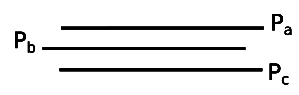
\includegraphics[width=4.5cm]{img/edge-clique.png} & &
    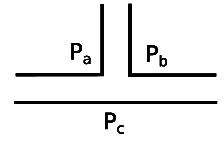
\includegraphics[width=3.5cm]{img/claw-clique.png}%b1EpgTransparenteGrade2
    \\
    \footnotesize %\centering 
    (a)  \footnotesize Representation of a clique as edge-clique. && \footnotesize (b) Representation  of a clique as claw-clique.\\
  \end{tabular}

 \caption{Examples of clique representations.} \label{fig:cliquesRepresentation}
\end{figure}    

Notice that if three vertices induce a claw-clique, then exactly two of them turn at the center of the corresponding  claw of the grid, and the third one contains the
base of the claw. 
Furthermore, any other vertex  adjacent to the three  must contain two of the edges of that claw, then the following lemma holds.

\begin{lema}\label{lem:cliquesMaximais}
If three vertices are together  in more than one maximal clique of a graph $G$, then in
any $B_1$-EPG representation of $G$ the three vertices do not form a claw-clique. %corresponding paths do not form a claw.
\end{lema}

\begin{figure}[ht]
  \centering
  \begin{tabular}{  p{5cm} p{0.7cm} p{5cm} }
    %\centering
    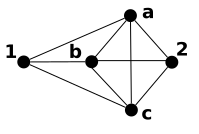
\includegraphics[width=3.5cm]{img/lemaClaw2Maximais} & &
    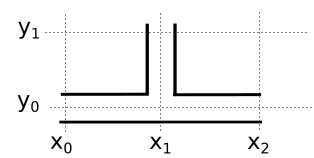
\includegraphics[width=5.5cm]{img/claw2}
    \\
    \footnotesize %\centering 
    (a)  \footnotesize Example of two maximal cliques sharing vertices. && \footnotesize (b) Representation  of a claw-clique in grid.\\
  \end{tabular}

 \caption{Vertices represented by a claw are present in a unique maximal clique.} \label{fig:lemaClaw2Maximais}
\end{figure}

In \cite{ries2009} Asinowski et al. proved the following lemma for $C_4$-free graphs.

\begin{lema} \cite{ries2009} \label{lem:lemaBRies2009}
Let $G$ be a $B_1$-EPG graph. If $G$ is $C_4$-free, then there exists a $B_1$-EPG representation of $G$ such that every  maximal claw-clique $K$ is represented on a claw of the grid whose base is covered only by vertices of $K$.
\end{lema}


We have obtained the following similar result for diamond-free graphs. A \textit{diamond} is a graph $G$ with vertex set $V(G) = \{a, b, c, d\}$ and edge set $E(G)=\{ab, ac,bc, bd,cd\}$ (see Figure~\ref{fig:diamond}). %A graph is diamond-free if it does not contain a diamond as induced subgraph.

 \begin{figure}[htb]	
 \center%6.3
 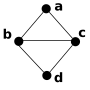
\includegraphics[width=2.2cm]{./img/diamond.png}
 \caption{Diamond graph.}
\label{fig:diamond}
\end{figure}  
 


\begin{lema}\label{lem:b1epgDiamondFree}
Let $G$ be a $B_1$-EPG graph. If $G$ is diamond-free, then in any $B_1$-EPG representation of $G$,  every maximal claw-clique $K$ is represented on a claw of the grid whose edges are covered only by vertices of $K$.
\end{lema}

\begin{proof}Let $K$ be a maximal clique which is a claw-clique in a given $B_1$-EPG representation of $G$. Then there exist three vertices of $K$ which induce a claw-clique $K'$ on
the same claw of the grid than $K$. Assume, in order to derive a contradiction, that a vertex $v\notin K$ covers some edges of the claw. Clearly, $v$ must  cover
only one of such edges. Therefore $v$ and the vertices of $K'$ induce a diamond, a contradiction. $\square$
\end{proof}


% \begin{defi} \label{defi:tortasFrame}

Let $ Q $ be a grid and let $ (a_1, b),$ $(a_2, b),$ $(a_3, b),$ $(a_4, b)$ be a $4$-star centered at $b$ as depicted in Figure~\ref{fig:piesInGrid}(a). Let $ \mathcal{P} = \{P_1, \dots , P_4\}$ be a collection of four paths each containing a different pair of edges of the $4$-star.
%exactly two edges of the $4$-star:
Following \cite{golumbic2009}, we say that the four paths form
\begin{itemize}
\item a \emph{true pie} %is a representation where each $P_i$ of $ \mathcal{P} $ has a bend at $b$.
when each one has a bend at $b$, Figure~\ref{fig:piesInGrid}(b); and 
\item a \emph {false pie} when exactly two of the paths %$P_i$  do not 
bend at $b$ and they do not share an edge of the $4$-star, FigureFigure~\ref{fig:piesInGrid}(c). %contain bends, while the remaining two do not share an edge. 

\begin{figure}[htb]
  \centering
%segundo bloco de figuras
  \begin{tabular}{c c c c c }
    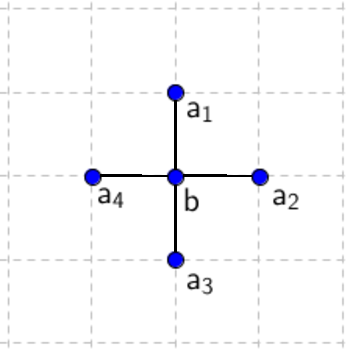
\includegraphics[width=3.5cm]{img/disposicaoTortaGrid3.pdf}    
    & &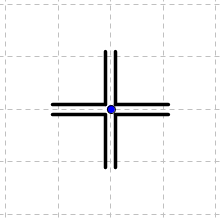
\includegraphics[width=3.5cm]{img/truePieGrid} 
    & &
 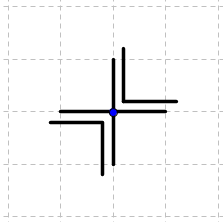
\includegraphics[width=3.5cm]{img/falsePieGrid} \\%[\abovecaptionskip]
    {\footnotesize (a) 4-star in grid.}  & &  {\footnotesize (b) True pie.} & & {\footnotesize (c) False pie.} 
  \end{tabular}
  \caption{$B_{1}$-EPG representation of the induced cycle of size 4 as pies with emphasis in center $b$.}\label{fig:piesInGrid}
\end{figure} 

%\vspace{-0.5cm}
\end{itemize}
% \end{defi}

Clearly if four paths of a $B_1$-EPG representation of $G$ form a pie, then the corresponding vertices induce a $4$-cycle in $G$. % The converse implication is also true (see~\cite{golumbic2009}). 
The following result can be easily proved. We say that a set of paths form a claw when each pair of edges of the claw is covered by some of the paths.

\begin{lema}\label{lem:twoClawNotSameCenterInChordal}
In any $B_1$-EPG representation of a graph $G$, a set of paths forming two different claws centered at the same point of the grid contains four paths forming either a true pie or a false pie. Therefore, in any $B_1$-EPG representation of a chordal graph $G$, no two maximal claw-cliques of $G$ are centered at the same point of the grid.
\end{lema}

\begin{lema}\label{lem:3cliquesNotClaw}
Let $G$ be a graph whose vertex set  can be
partitioned into a non trivial clique $K$ and an independent set $I=\{w_1,w_2,w_3\}$, such that each vertex of $K$ is adjacent to each vertex of $I$. Then, in any $B_1$-EPG representation of $G$, at least one of the cliques  $K_i = K \cup \{w_i\}$, with $1 \leq i \leq 3$,  is an edge-clique. 
\end{lema}

\begin{proof}
Assume, in order to derive a contradiction, that the three cliques are claw-cliques. By Lemma~\ref{lem:twoClawNotSameCenterInChordal}, they have different centers, say the points $q_1, q_2, q_3$ of the grid, respectively. Since at least two paths have a bend at the center of a claw, for each $i\in\{1,2,3\}$,   there must exist a vertex
  $v_i$ of $K$ such that the corresponding path $P_{v_i}$ turns at the point $q_i$ of the grid.  Notice that each one of the three paths $P_{v_i}$
  must contain  the three grid points $q_1$, $q_2$ and $q_3$. To prove that this is not possible, we will consider, without loss of generality, two cases.
  First,  $q_1$ is between $q_2$ and $q_3$ in $P_{v_1}$. Then, $P_{v_3}$ cannot turn at $q_3$ and contain $q_1$ and $q_2$.   And second,
  $q_2$ is between $q_1$ and $q_3$ in $P_{v_1}$. In this case, $P_{v_2}$ cannot turn at $q_2$ and contain $q_1$ and $q_3$; thus the proof is completed.
 $\square$
\end{proof}

Three vertices $u, v, w$ of a graph $G$ form an \textit{asteroidal triple} (AT) of $G$ if for every pair of them there exists a path connecting the two vertices and such that the path avoids the neighborhood of the remaining vertex~\cite{Asinowski2009}. A graph without an asteroidal triple is called \textit{AT-free}. 

\begin{lema}
[\cite{ries2009}] \label{l:AT-free} Let $v$ be any vertex of a $B_1$-EPG graph $G$. Then $G[N(v)]$ is AT-free.
\end{lema}

Let $C$ be any subset of the vertices of a graph $G$. The \textit{branch graph} $B(G|C)$, see~\cite{golumbic2009}, of $G$ over $C$ has a vertex set, $V(B)$, consisting of all the vertices of $G$ not in $C$ but adjacent to some member of $C$, i.e. $V(B) = N(C) - C$. Adjacency in $B(G|C)$ is defined as follows: we join two vertices $x$ and $y$ by an edge in $E(B)$ if and only if in $G$ occurs:
\begin{enumerate}
    \item  $x$ and $y$ are not adjacent;
    \item $x$ and $y$ have a common neighbor $u \in C$;
    \item the sets $N(x) \cap C$ and $N(y) \cap C$ are not comparable, i.e. there exist private neighbors $w, z \in C$ such that $w$ is adjacent to $x$ but not to $y$, and $z$ is adjacent to $y$ but not to $x$; we say that $x$ and $y$ are neighborhood incomparable.
\end{enumerate}

A graph $G$ is \textit{k-colorable} if its vertices can be colored with at most $k$ colors in such a way that no two adjacent vertices share the same color. 

\begin{lema}[~\cite{golumbic2009}] \label{l:branch} Let $C$ be any maximal clique of a $B_1$-EPG  graph $G$. Then, the branch graph $B(G|C)$ is $\{P_6, \, C_n \hbox{ for }  n\geq 4\}$-free.
\end{lema}





\section{Subclasses of Helly $B_1$-EPG Graphs}

In this section, we delimit some  subclasses of $B_1$-EPG graphs that admit a Helly $B_1$-EPG representation. It is known that $B_1$-EPG and Helly $B_1$-EPG 
are hereditary classes, so they can  be characterized by forbidden structures. 
In both cases, finding the list of minimal forbidden induced subgraphs are challenging open problems.
Taking a step towards solving
those problems,  we describe a few structures % that  provide a $B_1$-EPG graph does not admit a Helly $B_1$-EPG representation, that is it is not a  Helly $B_1$-EPG graph. 
at least one of which will  necessarily be present in  any $B_1$-EPG graph that does not admit a Helly representation. 
In addition,
we show that the well known families of Block graphs, Cactus and Line of Bipartite graphs are totally contained in the class Helly $B_1$-EPG.


Let $S_{3}, S_{3'}, S_{3''}$ and $ C_{4}$ be the graphs depicted in Figure \ref{fig:proibidos}. 


\begin{theorem}
\label{lem:chordalDiamondFree}
Let $G$ be a $B_1$-EPG graph. If $G$ is  $\{S_{3}, S_{3'}, S_{3''}, C_{4}\}$-free then $G$  is a Helly $B_1$-EPG graph.
\end{theorem}

\begin{proof}
If $G$ is not a Helly $B_1$-EPG graph, then in each $B_1$-EPG representation of $G$, there is at least one clique that is represented as claw-clique and no as edge-clique. Consider any $B_1$-EPG  representation of $G$  and let $K$ be a maximal clique  which is represented as a claw-clique. Assume, w.l.o.g,  $K$ is on a claw of the grid with base $[x_0, x_2]\times\{y_0\}$ and center $C = (x_1, y_0)$. Denote by  $\mathcal{P}_K$ the set of paths corresponding to the vertices of $K$.  By Lemma~\ref{lem:lemaBRies2009},  %(see~\cite{ries2009})
%no path $P_w$ for $w\notin K$ covers 
the grid segment $[x_0, x_2]\times\{y_0\}$ is covered only by vertices of $K$. % because $G$ is $C_4$-free


 For every ${\displaystyle \lrcorner}$-path %$P_v \in \mathcal{P}_K$ 
 (resp. ${\displaystyle \llcorner}$-path 
% $P_{v'} \in \mathcal{P}_K$
 ) belonging to $\mathcal{P}_K$, we do the following: if %$P_v$ (resp. $P_{v'}$)
 the path does not intersect any path $P_t \notin\mathcal{P}_K$ on column $x_1$, then we delete its vertical segment and add the grid segment $[x_1, x_2]\times\{y_0\}$ (resp. $[x_0, x_1]\times\{y_0\}$). If after this transformation there is no more ${\displaystyle \lrcorner}$-paths (resp. ${\displaystyle \llcorner}$-paths) in $\mathcal{P}_K$, then we are done since we have obtained an edge-clique. So we may assume that
 every ${\displaystyle \lrcorner}$-path   and every ${\displaystyle \llcorner}$-path  in $ \mathcal{P}_K$ intersects some path $P_t \notin \mathcal{P}_K$   on column $x_1$ (notice that we can assume is the same path $P_t$ for all the vertices). 
 
 Now, if none of the ${\displaystyle \lrcorner}$-paths belonging to $\mathcal{P}_K$ intersects  a path non in  $ \mathcal{P}_K$ on the line $y_0$, then we can replace the horizontal part of those paths by the segment $[x_1,x_2]\times \{y_0\}$, getting an edge representation of the clique $K$. Thus, we can assume there exists
 at least one ${\displaystyle \lrcorner}$-path $P_{v} \in \mathcal{P}_K$ intersecting some path  $P_{t'} \notin \mathcal{P}_K$ on line $y_0$. Analogously, there exists
 at least one ${\displaystyle \llcorner}$-path $P_{v'} \in \mathcal{P}_K$ intersecting some path  $P_{t''} \notin K$ on line $y_0$, as depicted in Figure~\ref{fig:clawGrid}. Notice that vertex $t'$ cannot be adjacent to any of the vertices $t$, $v'$ or $t''$; and, in addition, vertex $t''$ cannot
 be adjacent to   $t$,  or $v$.
 
 Finally,   since $K$ is claw-clique,  there is a path $P_u \in \mathcal{P}_K$ covering the base of the claw. Depending on the 
 possibles adjacencies between  $u$ and $t'$ or  $t''$, one of the graphs  $S_{3}$, $S_{3'}$ or $S_{3''}$ is obtained.
$\square$
\end{proof}


\begin{figure}[h]
  \centering
  \begin{tabular}{  c p{0.7cm} c}
    %\centering
    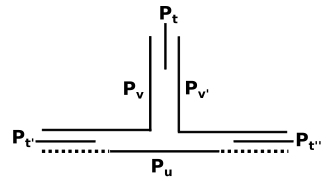
\includegraphics[width=5.5cm]{img/clawGrid} & &
    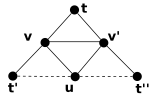
\includegraphics[width=3.5cm]{img/clawInduced.png}
    \\
    \footnotesize %\centering 
    (a)  \footnotesize Claw with paths. && \footnotesize (b) Subgraph induced by paths.\\
  \end{tabular}

 \caption{Reconstruction of the intersection model.}
 \label{fig:clawGrid}
\end{figure} 

 



Notice that any bull-free graph is $\{S_{3}, S_{3'}, S_{3''}\}$-free, so our previous result implies  Lemma 5 of  \cite{ries2009}.


\begin{figure}[h]
  \centering
  \begin{tabular}{  c p{0.7cm} c }
    \centering
    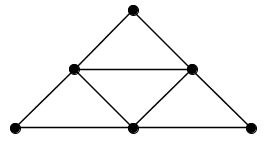
\includegraphics[width=4cm]{img/s3.png} & &
    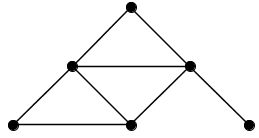
\includegraphics[width=4cm]{img/s3-1.png}
    \\
    \footnotesize \centering 
    (a)  \footnotesize Graph $S_3$. &&  \footnotesize (b) Graph $S_{3'}$. \\
    
    %---------------------
      \centering 
      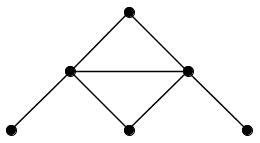
\includegraphics[width=4cm]{img/s3-2.png} & &
    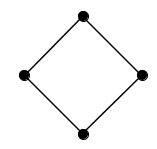
\includegraphics[width=3cm]{img/c4.png}
    \\
    \footnotesize \centering 
    (c)  \footnotesize Graph $S_{3''}$. && \footnotesize (b) Graph $C_{4}$.\\
  \end{tabular}

 \caption{Graphs on the statement of Theorem \ref{lem:chordalDiamondFree}.}
 \label{fig:proibidos}
\end{figure} 



%--------------------------


Next theorem has as consequence the identification of several graph classes where the existence of a $B_1$-EPG representation ensures the existence of a Helly $B_1$-EPG representation.


\begin{theorem} \label{lem:b1DiamondFree}
 If $G$ is a $B_1$-EPG and diamond-free graph then $G$ is a Helly $B_1$-EPG graph.
 \end{theorem}

\begin{proof}
If $G$ is not a Helly $B_1$-EPG graph, then in each $B_1$-EPG representation of $G$, there is at least one clique that is represented as claw-clique and no as edge-clique.  Consider any $B_1$-EPG  representation of $G$  and let $K$ be a maximal clique  which is represented as a claw-clique. Assume, w.l.o.g,  $K$ is on a claw of the grid with base $[x_0, x_2]\times\{y_0\}$ and center $C = (x_1, y_0)$. Denote by  $\mathcal{P}_K$ the set of paths corresponding to the vertices of $K$. 
 By Lemma~\ref{lem:b1epgDiamondFree},  %(see~\cite{ries2009})
%no path $P_w$ for $w\notin K$ covers 
the grid segment $[x_0, x_2]\times\{y_0\}$ is covered only by vertices of $K$. % because $G$ is $C_4$-free
 For every ${\displaystyle \lrcorner}$-path %$P_v \in \mathcal{P}_K$ 
 (resp. ${\displaystyle \llcorner}$-path 
% $P_{v'} \in \mathcal{P}_K$
 ) belonging to $\mathcal{P}_K$, we do the following: if %$P_v$ (resp. $P_{v'}$)
 the path does not intersect any path $P_t \notin\mathcal{P}_K$ on column $x_1$, then we delete its vertical segment and add the grid segment $[x_1, x_2]\times\{y_0\}$ (resp. $[x_0, x_1]\times\{y_0\}$). If after this transformation there is no more ${\displaystyle \lrcorner}$-paths (resp. ${\displaystyle \llcorner}$-paths) in $\mathcal{P}_K$, then we are done since we have obtained an edge-clique. So we may assume that
 every ${\displaystyle \lrcorner}$-path   and every ${\displaystyle \llcorner}$-path  in $ \mathcal{P}_K$ intersects some path $P_t \notin \mathcal{P}_K$   on column $x_1$ (notice that we can assume is the same path $P_t$ for all the vertices). Since  $K$ is claw-clique,  there is a path $P_u \in \mathcal{P}_K$ covering the base of the claw. Thus, $G[v, v', u, t]$ induces a diamond,  a contradiction. $\square$
\end{proof}  

An \textit{independent set} of vertices is a set of vertices no two of which are adjacent.
A graph $G$ is said to be \textit{Bipartite} if its set of vertices can be partitioned into two distinct independent sets.
 There are Bipartite graphs that are non $B_1$-EPG, for instance $K_{2,5}$ and $K_{3,3}$ (see~\cite{cohen2014}). Clearly , since
 bipartite graphs are triangle-free, any $B_1$-EPG representation of a bipartite graph is also a Helly $B_1$-EPG representation.
 A similar result (but a bit weaker) is obtained as corollary of the previous theorem. 


\begin{corollary}
If $G$ is a Bipartite $B_1$-EPG graph then $G$ is a Helly $B_1$-EPG graph.
\end{corollary}

\begin{proof}
The Bipartite graphs are diamond-free, thus by Theorem~\ref{lem:b1DiamondFree} these graphs are Helly $B_1$-EPG graphs.
\end{proof}

A \textit{Block graph} or \textit{Clique Tree} is a type of graph in which every biconnected component (block) is a clique.

\begin{corollary}\label{lem:cdf}
 Block graphs are Helly $B_1$-EPG.
\end{corollary}

\begin{proof}
Block graphs are known to be exactly the chordal diamond-free graphs, so by   Theorem 19 of \cite{ries2009}, all Block graphs are  $B_1$-EPG. If follows from Theorem~\ref{lem:b1DiamondFree} that all Block graphs are Helly $B_1$-EPG. 
 $\square$\end{proof} 

A \textit{Cactus} (sometimes called a cactus tree)  graph is a connected graph in which any two  cycles have at most one vertex in common. Equivalently, it is a connected graph in which every edge belongs to at most one  cycle, or (for nontrivial cactus) in which every block (maximal subgraph without a cut-vertex) is an edge or a cycle. The family of graphs in which each component is a cactus is closed under graph minor operations. This graph family may be characterized by a single forbidden minor, the diamond graph.
 
\begin{corollary}
Cactus graphs are  Helly $B_1$-EPG.
\end{corollary}
\begin{proof}
In~\cite{cela2019monotonic}, it is proved that every Cactus graph is a monotonic $B_1$-EPG graph 
(there is a $B_1$-EPG representation where all paths are ascending in rows and columns). 
Thus, Cactus graphs are $B_1$-EPG graphs. 

Since Cactus are diamond-free, by Theorem ~\ref{lem:b1DiamondFree}, the proof follows.
$\square$\end{proof}

Given a graph $G$, its \textit{Line graph} $L(G)$ is a graph such that each vertex of $L(G)$ represents an edge of $G$ and
  two vertices of $L(G)$ are adjacent if and only if their corresponding edges share a common endpoint (i.e. ``are incident'') in $G$.  
A graph $G$ is a \textit{Line graph of a Bipartite graph} (or simply \textit{Line of Bipartite}) if and only if it
contains no claw, no odd cycle, and no diamond as induced subgraph, \cite{harary1974line}.



\begin{corollary}\label{coro:lineOfBipartite}
 Line of Bipartite graphs are Helly $B_1$-EPG. 
\end{corollary}

\begin{proof}
Line of Bipartite graphs were proved to be $B_1$-EPG in~\cite{golumbic2018edge}. Since they are diamond-free, the proof follows from Theorem~\ref{lem:b1DiamondFree}.
$\square$
\end{proof}

The diagram of Figure~\ref{fig:diagram}
illustrates the containment relationship between the graph classes  studied so far in this work. 
We list in Figure~\ref{fig:exemplosDiagram} examples of graphs in each numbered region of the diagram. The numbers of each item below correspond to the regions of the same number in the diagram depicted in Figure~\ref{fig:diagram}.

%This numbers correspond with the respective number item and in some cases we make a brief explanation.

\begin{enumerate}[label=(\arabic*)]
    \item $B_1$-EPG  - Helly $B_1$-EPG graphs, depicted in Figure~\ref{fig:exemplosDiagram}(a), graph $E_1$;%1
    
    \item Line of Bipartite graphs  - Cactus - Block - Bipartite graphs, depicted in Figure~\ref{fig:exemplosDiagram}(b), graph $E_2$;%2
    \item Helly $B_1$-EPG - Line of Bipartite - Block - Cactus - Bipartite graphs, depicted in Figure~\ref{fig:exemplosDiagram}(c), graph $E_3$;%3
    \item Block $\cap$ Line of Bipartite - Cactus - Bipartite, depicted in Figure~\ref{fig:exemplosDiagram}(d), graph $E_4$;%4
    \item Block $\cap$ Line of Bipartite $\cap$  Cactus - Bipartite, depicted in Figure~\ref{fig:exemplosDiagram}(e), graph $E_5$;%5
    \item Cactus $\cap$ Line of Bipartite - Block - Bipartite. This intersection is empty. Let $G$ be a graph that is Cactus and Line of Bipartite then $G$ is $\{$claw, odd cycle, diamond$\}$-free. But $G$ is not a Bipartite graph, then $G$ has odd cycle. Thus $G$ has at least one triangle, at least one cycle $C_n, n\geq 4$, and $G$ is a connected graph. But given a cycle $C_n, n\geq 4$, if add one vertex any adjacent to this cycle then this induce a claw, absurd with the hypothesis of $G$ is Line of Bipartite;%6
    \item Bipartite $\cap$ Line of Bipartite  - Cactus - Block graphs, depicted in Figure~\ref{fig:exemplosDiagram}(f), graph $E_7$;%7
    \item Bipartite $\cap$ Line of Bipartite $\cap$  Cactus - Block graphs, depicted in Figure~\ref{fig:exemplosDiagram}(g), graph $E_8$;%8
    \item Bipartite $\cap$ Line of Bipartite $\cap$  Cactus $\cap$ Block graphs, depicted in Figure~\ref{fig:exemplosDiagram}(h), graph $E_9$;%9
  \item Bipartite $\cap$  Cactus $\cap$ Block - Line of Bipartite graphs, depicted in Figure~\ref{fig:exemplosDiagram}(i), graph $E_{10}$;%10
    \item Bipartite  $\cap$  Cactus - Block -  Line of Bipartite graphs, depicted in Figure~\ref{fig:exemplosDiagram}(j), graph $E_{11}$;%11
     \item Bipartite $\cap$ Helly $B_1$-EPG - Cactus - Block -  Line of Bipartite graphs, depicted in Figure~\ref{fig:exemplosDiagram}(k), graph $E_{12}$;%12
      \item Bipartite - $B_1$-EPG graphs, depicted in Figure~\ref{fig:exemplosDiagram}(l), graph $E_{13}$;%13
      \item Block - Bipartite - Line of Bipartite  - Cactus graphs, depicted in Figure~\ref{fig:exemplosDiagram}(m), graph $E_{14}$;%14
 
      \item Block $\cap$  Cactus -  Line of Bipartite - Bipartite graphs, depicted in Figure~\ref{fig:exemplosDiagram}(n), graph $E_{15}$;%15
      \item Cactus - Block -  Line of Bipartite - Bipartite graphs, depicted in Figure~\ref{fig:exemplosDiagram}(o), graph $E_{16}$, the odd cycles $C_{2n+1},n\geq 2$;%16
      \item Helly EPG - $B_1$-EPG  - Bipartite graphs, depicted in Figure~\ref{fig:exemplosDiagram}(p), graph  $E_{17}$;%17
\end{enumerate}



 \begin{figure}[htb]	
 \center%6.3
 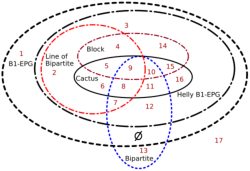
\includegraphics[width=8cm]{./img/diagram.pdf}
 \caption{Diagram of some graph classes.}
\label{fig:diagram}
\end{figure}  
 


 \begin{figure}[htb]	
 
   \centering
  \begin{tabular}{  c c c c  c}
    %\centering
    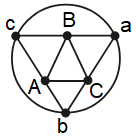
\includegraphics[width=3cm]{img/octaedro.png} 
    & 
    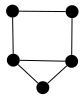
\includegraphics[width=1.5cm]{img/ex3.png} 
    & 
    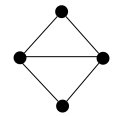
\includegraphics[width=2cm]{img/diamondNoLabel.png} 
    & 
    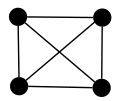
\includegraphics[width=1.5cm]{img/k4.png} 
    & 
    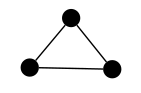
\includegraphics[width=2cm]{img/k3.png} 
    \\
    \footnotesize 
    (a)  \footnotesize Graph $E_1$. 
    & 
    \footnotesize (b) Graph $E_2$.
    & 
    \footnotesize (c) Graph $E_3$.
    & 
    \footnotesize (d) Graph $E_4$.
    & 
    \footnotesize (e) Graph $E_5$.
    \\%%Segunda linha
        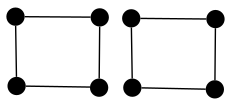
\includegraphics[width=2.5cm]{img/2c4.png} 
    & 
    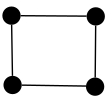
\includegraphics[width=1.5cm]{img/c4e.png} 
    & 
    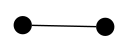
\includegraphics[width=1.8cm]{img/k2.png} 
    & 
    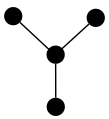
\includegraphics[width=1cm]{img/e10.png} 
    & 
    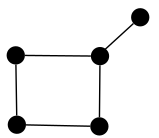
\includegraphics[width=1.8cm]{img/e11.png} 
    \\ %%Segundo Bloco legendas
    \footnotesize 
    (f)  \footnotesize Graph $E_7$. 
    & 
    \footnotesize (g) Graph $E_8$.
    & 
    \footnotesize (h) Graph $E_9$.
    & 
    \footnotesize (i) Graph $E_{10}$.
    & 
    \footnotesize (j) Graph $E_{11}$.
    %%Terceira linha de imagens
    \\%%Terceira linha
        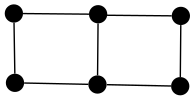
\includegraphics[width=2.5cm]{img/e12.png} 
    & 
    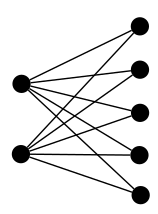
\includegraphics[width=2cm]{img/k25.png} 
    & 
    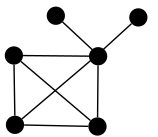
\includegraphics[width=2cm]{img/e14.png} 
    & 
    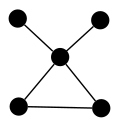
\includegraphics[width=1.8cm]{img/e15.png} 
    & 
    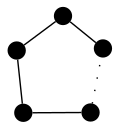
\includegraphics[width=1.8cm]{img/c2n+1.png} 
    \\ %%Terceiro Bloco legendas
    \footnotesize 
    (k)  \footnotesize Graph $E_{12}$. 
    & 
    \footnotesize (l) Graph $E_{13}$.
    & 
    \footnotesize (m) Graph  $E_{14}$.
    & 
    \footnotesize (n) Graph $E_{15}$.
    & 
    \footnotesize (o)  Graph $E_{16}$,  $C_{2n+1},n\geq2$.
    \\
    &&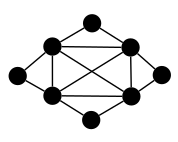
\includegraphics[width=2.5cm]{img/4sunNoLabel.png}&&
    \\
    &&\footnotesize (p)  Graph $E_{17}$.&&
    
    %\multicolumn{3}{c}{ \footnotesize (c) Another partial single bend representation of $H$ } \\
  \end{tabular}
 \caption{The set of instances for Venn Diagram of the graph classes of this paper.}
 %, see  more in~\cite{leveque2009characterizing,tondato2009grafos}
 \label{fig:exemplosDiagram}
\end{figure}  
 

\section{Containment relationship between Chordal $B_1$-EPG, VPT and EPT graphs }


 Any graph that
admits a $B_1$-EPG representation  whose paths do not cover all the edges of a polygon of the grid (i.e.
the subjacent grid subgraph is a tree)  is also an EPT graph: the same representation is both $B_1$-EPG and $EPT$.
However, it is easily verifiable that the subjacent grid subgraph of any $B_1$-EPG representation of a cycle $C_n$ with $n\geq 5$ is not a tree,
%has a non chordal subjacent grid subgraph 
although $C_n$ is an  EPT graph.  Our long-rage goal is 
understanding the $B_1$-EPG graphs that are also EPT graphs. When can a $B_1$-EPG representation
be reorganized into an EPT representation?  In this section,
 we answer that question for Chordal $B_1$-EPG graphs, in fact we prove that every Chordal $B_1$-EPG graph is EPT. We
 made several unsuccessful attempts to prove this result by considering for a graph $G$, a $B_1$-EPG representation whose paths cover all the edges
 of some polygon on the grid, and trying  to show  that if none of the paths could be modified in order to avoid an edge of the polygon,
 then $G$ had some chordless  cycle (i.e. $G$ is not chordal). The surprise was that the only way we found to demonstrate our main Theorem \ref{teo:b1epgept} was through $VPT$ graphs.
 We will prove the following theorem.

\begin{theorem}\label{teo:chordalB1inVPT}
Chordal $B_1$-EPG $\subsetneq$ VPT. 
\end{theorem}

In~L{\'e}v{\^e}que et al. \cite{leveque2009characterizing} apud \cite{alcon2015characterizing},  VPT graphs were characterized by a family of minimal forbidden induced subgraphs,
the ones depicted in 
Figure~\ref{fig:16proibidos} plus the induced cycles $C_n$ for $n\geq 4$. Therefore, in order to prove
that Chordal $B_1$-EPG graphs are VPT is enough to show that none of the graphs in Figure~\ref{fig:16proibidos} 
is $B_1$-EPG. %The following lemmas are developed with that objective.   

First notice that in each one of the graphs $F_{1}, F_{2}, F_{3}, F_{4}$ and $F_{5}$ ( Figures~\ref{fig:16proibidos}(a), (b), (c), (d), (e), respectively), the neighborhood of the universal vertex (the one that is a bit bigger than the others, in the respective figures) contains an asteroidal triple. Therefore, by Lemma \ref{l:AT-free}, these graphs are not  $B_1$-EPG.

Now, in each one of the graphs $F_{11}, F_{12}, F_{13}, F_{14}$, $F_{15}$ and $F_{16}$  (Figures~\ref{fig:16proibidos}(k), (l), (m), (n), (o), (p), respectively), let $C$ be the maximal clique in bold. It is easy to check that, in all cases, the branch graph $B(G|C)$ contains an induced cycle $C_n$, for some $n\geq 4$, or an induced path $P_6$; thus, by Lemma \ref{l:branch},  graphs $F_{11}, F_{12}, F_{13}, F_{14}$, $F_{15}$ and $F_{16}$ are not $B_1$-EPG.



  A \textit{satellite} of a clique $K$ is a vertex $v$ such that $B_v=N(v)\cap K$ is a 
nonempty proper subset of $K$. The set $B_v$ is called the \textit{base} of $v$ and it is said \textit{minimal} if no other
base of a satellite of $K$ is properly contained in $B_v$, see~\cite{alcon2010necessary}.

 Let $I=[q_1,q_2]$ be the grid interval defined by the intersection $\displaystyle \cap_{v\in K}P_v$, where $K$
is an edge-clique of a graph $G$. For any $v\in K$, by removing the interval $(q_1,q_2)$, the path $P_v$
is split into two \textit{disjoint parts}: \textit{part 1}  containing $q_1$, and  \textit{part 2}  containing $q_2$.
If $w$  is a satellite of $K$ adjacent to $v$, then
$P_w\cap P_v$ is contained either in part 1 or in part 2 of $P_v$. We will say that $P_w$ intersects $P_v$
on side 1 or on side 2 of $K$, respectively. Notice that if $w$  is also adjacent
to another vertex $v'$ of $K$, then   $P_w$ intersects $P_v$ and $P_{v'}$ on
a same side of $K$. It allow us to divide the satellites of $K$ into two \textit{disjoint
groups}, the ones on  \textit{side 1} of $K$ and the ones on \textit{side 2}.

%%%%%%%%%%%%%%%%%%%%%%%%%%%
\begin{fac} \label{f:between}Let $e_1$, $e_2$ and $e_3$  be three distinct edges of a  one-bend path $P$, and assume that $e_2$ is between $e_1$ and $e_3$ on $P$. If $P_1$ and $P_3$ are one-bend paths such that: $P_1$ contains $e_1$, $P_3$ contains $e_3$, and  $P_1$ and $P_3$ intersect in at least one edge, then $P_1$ or $P_3$ contains $e_2$.
\end{fac}
%%%%%%%%%%%%%%%%%%%%%%%%%%%%%%

\begin{lema}\label{coro:3Cliques1EdgeClique}
Let $G$ be a graph whose vertex set  can be partitioned into a non trivial clique $K$ and an independent set $I=\{w_1,w_2,w_3\}$, such that each vertex of $K$ is adjacent to each vertex of $I$. Let $K_i$ be each maximal clique  $K_i = K \cup w_i$, with $1 \leq i \leq 3$.
In any $B_1$-EPG representation of $G$, one of those cliques, we say $K_2$, is an edge clique, and its two  satellites $w_1$ and $w_3$ are
on different sides.
\end{lema}

\begin{proof}
%%%%%%%%%%%%%%%%%%%%%%%%%%%%%%%
Let $v$ be any vertex of $K$. For $i\in \{1,2,3\}$, let $I_{v,i}$ be the subpath of $P_v$
defined to be $P_v\cap P_{w_i}$ (we  consider paths as edge sets). Clearly, the three
subpaths are pairwise edge-disjoint. Thus, w.l.o.g., by symmetry, we can assume that
$I_{v,2}$ is between  $I_{v,1}$ and $I_{v,3}$. We claim that the clique $K_2$ is an edge-clique.
Indeed, if it not, % then $P_4$ contains no edge of the subpath $I_{1,4}$. And,
by Lemma \ref{lem:3cliquesNotClaw}, we can assume, w.l.o.g., that $K_1$ is an edge clique, which implies that there is an edge of $I_{v,1}$ covered by all the vertices of $K_1$.  Let $q$ be the center of the claw corresponding to the clique $K_2$; clearly $q$ is a point of $I_{v,2 }$. Since all the vertices of $K$ must contain $q$, but not all them can cover a same
edge  of  $I_{v,2}$, we have that $q$ must be the extreme of  $I_{v,2}$ closest to  $I_{v,1}$. Therefore, if we let $e_1$ and $e_2$ be the two edges of $P_v$ incident on $q$ ($e_2$ the one contained in $I_{v,2}$),
we have that  all the vertices of $K$
contain  $e_1$ and at least one vertex of $K$, say $w$,  does not contain $e_2$. Observe this contradicts Fact \ref{f:between} (let $P_1=P_w$, $P_3=P_{w_3}$ and $e_3$ any edge of $I_{v,3}$. We conclude that $K_2$ is an edge clique; since $w_1$ and $w_3$ are satellites of $K_2$ the proof is complete. 
$\square$
%%%%%%%%%%%%%%%%%%%%%%%%%%%%%%%%%%%%%%%%%%%%%%%
% By Lemma~\ref{lem:3cliquesNotClaw} the maximal cliques $K_1, K_2$ and $K_3$ can not be represented simultaneously as claw-cliques, thus at least one is edge-clique, we say $K_2$. Since $G$ is a Chordal graph, then when $K_1$ and $K_3$ are represented as claw-cliques they have  distinct centers.
% Given $\mathcal{P}_K$ the set of paths corresponding to the vertices of $K$. 
% Each claw-clique $K_i$ has at least one path $P_k \in \mathcal{P}_K$ that bend in this claw-clique. If all paths $P_k \in \mathcal{P}_K$ bend in some claw-clique then these paths can not bend in other claw-clique, i.e. if all paths $P_k \in \mathcal{P}_K$ bend in some claw-clique others cliques will be edge-clique and the lemma holds. So, consider $K_1$ and $K_3$ as claw-cliques.
% In each claw-clique $K_1, K_3$, either all paths $P_k \in \mathcal{P}_K$ intersect in some segment between center of claw-clique and right or left part of base, or then there is only one point of intersection of all paths (center of this claw, obviously) and there is no a $B_1$-EPG representation to $G$. Consider the first situation,  w.l.g. we say that $K_1$ has horizontal base in interval $(q_1,q_2)$ and that all paths $P_k \in \mathcal{P}_K$ intersect  at right of $q_2$. Then, $K_3$ with base in interval $(q_1'',q_2'')$ has same condition but with intersection of all paths at left of $q_1''$. Now we have a problem, if edge-clique $K_2$ is at left of the center of the $K_1$ then there is a path $P_k \in \mathcal{P}_K$ that bend in the center of $K_1$ such that this path is not in $K_2$, the same is true if $K_2$ is at right of $K_3$. 
% Therefore, in this construction $K_2$ must be between the center of $K_1$ and $K_3$. 

% Thus there is always an edge-clique $K_i$ located between two satellites $w_i$. 
\end{proof}
